% =====================================================================
% Cross-Modal Dual-Agent RL for Poetry + Music Recommendation
% Team: Ro'Yah, Jonathan, Ali
% CSI5340 / ELG5214 -- Group 4
% Submission: single-column, 11pt, 1 inch margins, 6-10 pages
%   (excluding References and Appendix)
% =====================================================================
\documentclass[11pt]{article}

% ---------- Page geometry ----------
\usepackage[letterpaper, margin=1in]{geometry}

% ---------- Core packages ----------
\usepackage[T1]{fontenc}
\usepackage[utf8]{inputenc}
\usepackage{lmodern}
\usepackage{microtype}
\usepackage{graphicx}
\usepackage{amsmath, amssymb, amsthm}
\usepackage{booktabs}
\usepackage{array}
\usepackage{multirow}
\usepackage{caption}
\usepackage{subcaption}
\usepackage{enumitem}
\usepackage{xcolor}
\usepackage{url}
\usepackage[hidelinks]{hyperref}
\usepackage[numbers,sort&compress]{natbib}
\usepackage{authblk}

% ---------- Figure paths ----------
\graphicspath{{figures/}{../figures/}}

% ---------- Title block ----------
\title{\textbf{Cross-Modal Dual-Agent Reinforcement Learning for\\
Emotion-Aligned Poetry and Music Recommendation}}
\author[1]{Ali Khreis\thanks{Contact: akhre083@uottawa.ca. Ali Khreis is a M.Eng.\ student at the University of Ottawa.}}
\author[1]{Jonathan Horton\thanks{Contact: jhort062@uottawa.ca. Jonathan Horton was a M.Eng.\ student at the University of Ottawa.}}
\author[1]{Ro'Yah Radaideh\thanks{Contact: rrada030@uottawa.ca. Ro'Yah Radaideh is a M.A.Sc.\ student at the University of Ottawa.}}
\affil[1]{University of Ottawa, CSI5340 / ELG5214, Group 4}
\date{24th of April 2026}

\begin{document}
\maketitle

% =====================================================================
% ABSTRACT
% =====================================================================
\begin{abstract}
We present a cross-modal recommender that aligns poetry and music in a
shared 128-dimensional emotion embedding space and uses two cooperating
reinforcement-learning agents to rerank short candidate slates. Text is
encoded with DistilBERT and projected into a joint space anchored by
valence-arousal signals derived from the Million Song Dataset; triplet
training yields cross-modal neighborhoods that respect mood rather than
surface features. On top of this representation we train two lightweight
world models (one per modality) to predict user engagement from synthetic
implicit feedback, and optimize item-conditional reranking policies with
REINFORCE and PPO against the learned simulator. Experiments on
Goodreads poetry and an MSD subset show that (i) the shared embedding
recovers meaningful valence-arousal structure, (ii) world models fit
engagement signals with stable validation loss, and (iii) the learned
policies improve over retrieval-only baselines by scoring candidates
based on session mood and user taste. This report addresses the following
research question: when does a reinforcement learning-based agent
outperform a simpler baseline on mood fit for music and book
recommendation?
\end{abstract}

% =====================================================================
% 1. INTRODUCTION & MOTIVATION
% =====================================================================
\section{Introduction and Motivation}
\label{sec:intro}

The number of multi-modal encoders has been increasing in recent years
due to the rising interest in multi-modal recommender
systems~\cite{xu2025survey}.

Recommender systems typically operate inside a single modality: a music
service ranks songs, a bookstore ranks books, and a video platform ranks
videos. Users, however, experience content through a unified emotional
lens: the poem that fits a rainy evening is often close in mood to the
song that fits it. This project asks a focused question: \emph{can two
recommender agents share a cross-modal emotion representation and
cooperatively improve engagement via reinforcement learning?}

We study this question in a compact, reproducible setting. Two catalogs
are used: Goodreads poetry and a subset of the Million Song Dataset
(MSD). Textual descriptions (book blurbs, track and artist context) are
encoded with DistilBERT and projected into a shared 128-dimensional
embedding trained with a triplet objective against valence-arousal
anchors. Each modality then has (a) a \emph{world model} that predicts
an engagement target from synthetic implicit feedback, and (b) an
\emph{item-conditional} policy that reranks a shortlist of candidates.
Policies are trained with REINFORCE and PPO against the world-model
simulator. A Gradio demo allows live interaction: user like/dislike
clicks are logged and used at inference time to personalize
recommendations, but do not retrain any model.

\paragraph{Contributions.}
\begin{enumerate}[leftmargin=*, itemsep=2pt]
    \item A \textbf{shared 128-d emotion space} that aligns poetry and
    music via triplet training with valence-arousal anchors
    (Section~\ref{sec:method-embedding}, implemented in
    \texttt{shared\_embedding.py}).
    \item Two \textbf{world models} trained offline on
    valence-arousal-derived synthetic feedback (100k rows each), with no
    real user logs (Section~\ref{sec:method-wm}, implemented in
    \texttt{music\_agent.py} and \texttt{book\_world\_model.py}).
    \item A \textbf{slate-bandit RL formulation} with an
    item-conditional reranker (\texttt{ItemScorerPolicy}) trained with
    REINFORCE and PPO against the world-model simulator
    (Section~\ref{sec:method-rl}, implemented in
    \texttt{train\_rl\_agents.py}).
    \item A \textbf{Gradio demo with a live GUI feedback loop}
    (\texttt{app.py}): user interactions are logged to
    \texttt{user\_history.csv} and used at inference to build a
    per-user taste vector, while the pretrained world model and policy
    remain frozen (Section~\ref{sec:method-gui}).
\end{enumerate}

\paragraph{Why this setup?}
Slate bandits over a small candidate list (rather than a softmax over
$\sim\!10^4$ items) give a clean MDP and stable gradients while still
capturing the core cross-modal coupling. Synthetic feedback tables
(\texttt{build\_feedback\_tables.py}) provide fully reproducible
training data; the GUI feedback loop (\texttt{user\_history.csv})
demonstrates inference-time personalization without requiring any
retraining.

\paragraph{Research question.}
When does a reinforcement learning-based agent outperform a simpler
baseline on mood fit for music and book recommendation?

% =====================================================================
% 2. RELATED WORK
% =====================================================================
\section{Related Work}
\label{sec:related}

\paragraph{Content-based and cross-modal representations.}
DistilBERT~\cite{sanh2020distilbert} and sentence transformers have
become standard text encoders for recommender content features. Joint
text-audio spaces built with contrastive or triplet losses extend this
idea~\cite{schroff2015facenet,radford2021clip}. Our embedding space
follows the structure of~\cite{Won2021emotion}, which maps embeddings
via $E_{\text{space}} = M\!\left(P_{\text{space}}(x)\right)$, where
\emph{space} is either music or text in our project. The modality gap
has been bridged using a variety of techniques: deep learning and common
representation spaces is the most common approach~\cite{yao2015ranking},
and canonical correlation analysis has also been
used~\cite{zhen2019cross}. Our use of valence-arousal anchors follows
the affective-computing tradition of the circumplex model of
affect~\cite{russell1980circumplex} and MSD-derived mood
labels~\cite{bertinmahieux2011msd}.

\paragraph{World models and model-based RL.}
World models learn a differentiable simulator of the environment and
enable policy optimization via imagined rollouts~\cite{ha2018world,
hafner2020dreamer}. In recommendation, this mirrors user simulator
approaches~\cite{shi2019virtualtaobao,ie2019recsim} where a learned
model replaces expensive online feedback. World models are commonly used
to simulate users, and are often trained using both online and offline
rewards~\cite{yao2015ranking}.

\paragraph{RL for recommendation and slate bandits.}
Policy-gradient and actor-critic methods have been adapted to ranking
tasks~\cite{chen2019topk,ie2019slateq}. PPO~\cite{schulman2017ppo} is a
popular on-policy algorithm; REINFORCE~\cite{williams1992reinforce}
offers a simpler baseline well suited to small slates. We combine the
slate-bandit framing with a world-model reward, following multi-agent
shared-state approaches~\cite{zou2020massa} adapted here for two
modalities. Reinforcement learning has also been applied directly to
emotion-based playlist generation~\cite{chi2010reinforcement}. Systems
like DJ-MC cluster songs by type and then apply Monte Carlo Tree Search
to the clustered catalog~\cite{liebman2014djmc}. Long-term online
studies have validated the value of recommender systems in commercial
deployment~\cite{shani2005mdp}, suggesting that a functional
emotional text-music recommender would likely be of commercial value.

% =====================================================================
% 3. METHODOLOGY
% =====================================================================
\section{Methodology}
\label{sec:method}

\subsection{Problem formulation}
\label{sec:method-problem}

Let $\mathcal{B}$ be the poetry catalog and $\mathcal{M}$ the music
catalog. A session state at step $t$ is the pair $s_t = (m_t, u_t) \in
\mathbb{R}^{128} \times \mathbb{R}^{128}$, where $m_t$ is the
\emph{mood embedding} (DistilBERT projection of the user prompt) and
$u_t$ is a \emph{user-taste vector}. During training, $u_t$ is a
randomly sampled embedding or zeros (simulating cold start). At
inference, $u_t$ is computed from the user's past likes in
\texttt{user\_history.csv} (see Section~\ref{sec:method-gui}). For
modality $X \in \{\mathcal{B},\mathcal{M}\}$, the agent observes $s_t$,
receives a candidate slate $A_t^X \subseteq X$ of size $K$ built by
retrieval, and chooses one item $a_t \in A_t^X$. The world model
$f_\phi^X$ predicts a scalar engagement reward $\hat r_t =
f_\phi^X(s_t, a_t)$, and the policy $\pi_\theta^X(a \mid s_t, A_t^X)$
is optimized to maximize expected reward.

\subsection{Shared emotion embedding}
\label{sec:method-embedding}

Textual content is encoded with DistilBERT~\cite{sanh2020distilbert} and
passed through a single-layer MLP projector ($768 \rightarrow 128$). We
anchor the space with valence-arousal tags derived from MSD mood
metadata~\cite{bertinmahieux2011msd}; poetry items are paired with
pseudo-VA labels mined from lexicon-based signals. A triplet loss
\[
\mathcal{L}_\text{trip} =
    \max\!\bigl(0,\;
        \|f(x)-f(x^+)\|_2 - \|f(x)-f(x^-)\|_2 + \alpha
    \bigr)
\]
with margin $\alpha{=}0.2$ pulls same-mood cross-modal pairs together.
Implementation: \texttt{shared\_embedding.py} (10 epochs, batch 32,
AdamW, lr $1{\times}10^{-4}$). Outputs: \texttt{poetry\_embeddings.npy}
and \texttt{music\_embeddings.npy}.

\subsection{World models and training data}
\label{sec:method-wm}

\paragraph{Training synthetic feedback.}
World models are trained entirely on synthetic data produced by
\texttt{build\_feedback\_tables.py} (100k rows per modality, 90/10
train/val split). Labels are computed from valence-arousal (VA) distance
with no real user logs involved: for music, skip and listen values are
derived from the VA distance between a randomly sampled poetry item and a
randomly sampled track; for books, rating and dislike values come from
the VA distance between two randomly sampled poetry items. Each row is
also assigned a synthetic user ID (round-robin across three names:
\emph{royah}, \emph{ali}, \emph{jonathan}) purely for organizational
splits; these IDs do not reflect real interactions. This data is
distinct from the GUI feedback described in
Section~\ref{sec:method-gui}.

\paragraph{Model architecture.}
Each world model is a 3-layer MLP over the concatenated mood and item
embedding $[m_t;\, e_{a_t}] \in \mathbb{R}^{256}$, with two sigmoid
heads trained with MSE loss. For music (\texttt{music\_agent.py}), the
heads predict \emph{skip probability} and \emph{listen time}. For books
(\texttt{book\_world\_model.py}), they predict \emph{rating} and
\emph{dislike probability}.

The world models serve two roles: (1) providing the reward signal during
RL training, and (2) optionally scoring the full catalog to build a
world-model-based candidate shortlist.

\subsection{Retrieval: building the candidate slate}
\label{sec:method-retrieval}

A retrieval stage selects $K{=}16$ candidates before the policy acts.
Three modes are implemented in \texttt{rl\_env.py}:
\begin{itemize}[leftmargin=*, itemsep=1pt]
    \item \textbf{Cosine}: top-$K$ by dot product between the unit mood
    vector and item embeddings.
    \item \textbf{MMR} (default, $\lambda{=}0.35$): maximal marginal
    relevance, which trades mood similarity for diversity so that slot~0
    is not always the cosine argmax.
    \item \textbf{World-model (WM)}: score every catalog item with the
    trained world model and take the top-$K$ by predicted engagement.
\end{itemize}
The retrieval mode is saved in the policy checkpoint so inference uses
the same logic as training.

\subsection{RL formulation: item-conditional reranker}
\label{sec:method-rl}

Given a slate $A_t = (e_1, \ldots, e_K)$ of item embeddings, the policy
is an \texttt{ItemScorerPolicy}: a small MLP that scores each candidate
conditioned on its embedding, not its slot index:
\[
    \pi_\theta(a_i \mid s_t, A_t)
    = \frac{\exp\!\bigl(\phi_\theta(s_t, e_i)\bigr)}
           {\sum_{j=1}^{K} \exp\!\bigl(\phi_\theta(s_t, e_j)\bigr)}.
\]
The score for item $i$ depends on the content of $e_i$, not its
position. Network architecture: $\text{Linear}(256{+}128 \rightarrow
128) \rightarrow \text{ReLU} \rightarrow \text{Linear}(128 \rightarrow
1)$.

Two optimizers are implemented in \texttt{train\_rl\_agents.py}:
\begin{itemize}[leftmargin=*, itemsep=1pt]
    \item \textbf{REINFORCE}~\cite{williams1992reinforce} with a
    running-mean baseline; lr $1{\times}10^{-3}$.
    \item \textbf{PPO}~\cite{schulman2017ppo} with clipped surrogate
    and a value head; lr $3{\times}10^{-4}$, clip $0.2$, 4 update
    epochs on a 64-step horizon.
\end{itemize}

The music reward combines world-model outputs with embedding-space
alignment:
\[
r = \alpha \cdot \text{listen}
  + \beta \cdot \cos(e_{\text{song}}, m_t)
  + \gamma \cdot \text{diversity}
  - \delta \cdot \text{skip},
\]
with $\alpha{=}0.35$, $\beta{=}0.35$, $\gamma{=}0.20$,
$\delta{=}0.10$. The book reward follows a similar structure using rating
and dislike heads. During training, $u_t$ is sampled randomly to
simulate a range of user preferences.

At inference (\texttt{policy\_inference.py}), the policy scores each
slate item, applies softmax, and reorders by descending probability.

\subsection{Gradio demo and GUI feedback}
\label{sec:method-gui}

The Gradio demo (\texttt{app.py}) is a live interface where users enter
their name, select a mood, and adjust an emotional intensity slider to
receive a recommended book and a playlist of 5 tracks. Like (+1) and
Dislike ($-1$) buttons on the top track log interactions to
\texttt{data/user\_history.csv} with columns: \texttt{timestamp},
\texttt{user}, \texttt{mood}, \texttt{item\_title}, \texttt{reward}.
This file is separate from the VA-distance synthetic training data.

The GUI feedback is used \emph{only at inference time} in two ways:
\begin{enumerate}[leftmargin=*, itemsep=1pt]
    \item \textbf{Taste vector} (\texttt{user\_preferences.py}): the
    liked items (reward $= 1$) for a given username are looked up and
    their embeddings are averaged to form $u_t$. New users receive
    $u_t = \mathbf{0}$ (cold start).
    \item \textbf{Personalized mood center} (\texttt{app.py}): the
    initial mood embedding $m_t$ is nudged 30\% toward the average
    embedding of the user's liked tracks to provide mild
    personalization.
\end{enumerate}
The world model and RL policy are \emph{not} retrained from this
feedback; the pretrained checkpoints remain fixed. The GUI feedback loop
therefore demonstrates lightweight inference-time personalization, not
online learning.

\subsection{Pipeline and reproducibility}
\label{sec:method-pipeline}

Figure~\ref{fig:pipeline} shows the full pipeline. All randomness is
controlled through \texttt{seed\_utils.py} and explicit \texttt{--seed}
flags on each training script.

\begin{figure}[h]
    \centering
    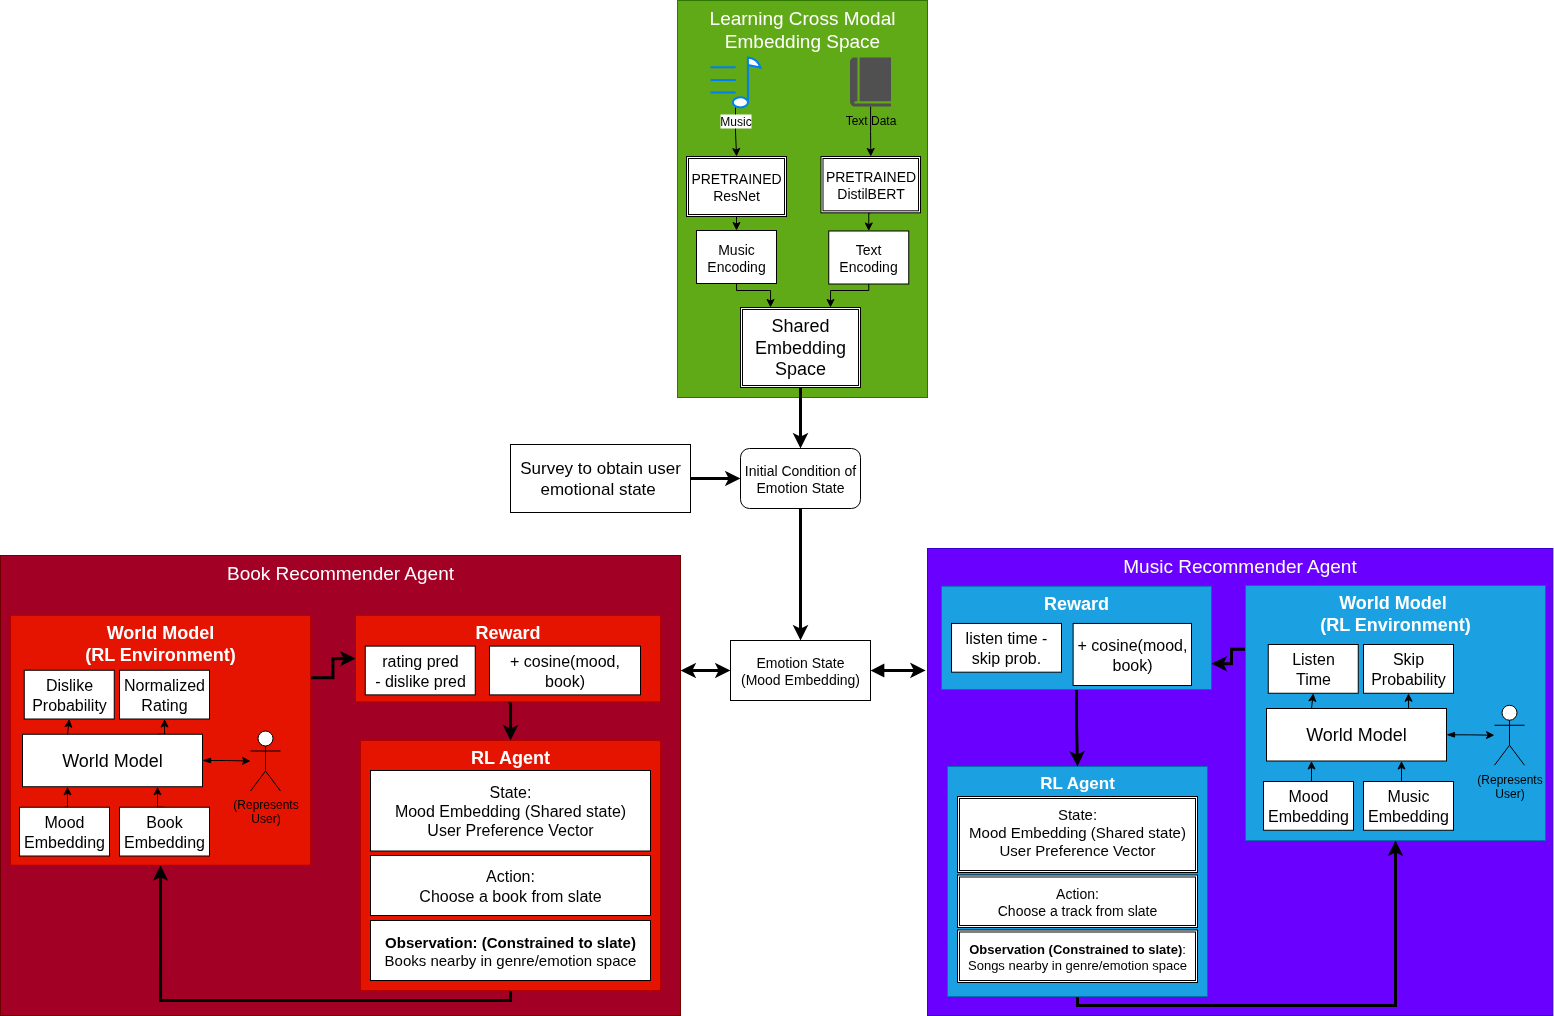
\includegraphics[width=\linewidth]{figures/pipeline.png}
    % \fbox{\parbox{0.85\linewidth}{\centering\vspace{1em}
    %     \textbf{Offline training:} catalogs $\rightarrow$ shared
    %     embedding $\rightarrow$ synthetic feedback tables $\rightarrow$
    %     world models $\rightarrow$ RL policies\\[0.5em]
    %     \textbf{Inference:} user prompt $\rightarrow$ mood embedding
    %     $+$ GUI taste vector $\rightarrow$ retrieval $\rightarrow$
    %     policy reranking $\rightarrow$ Gradio demo
    % \vspace{1em}}}
    \caption{End-to-end pipeline. Offline training (top) uses only
    VA-distance synthetic data. The GUI feedback loop (bottom) updates
    the inference-time taste vector but does not retrain any model.}
    \label{fig:pipeline}
\end{figure}

\subsection{Cosine baseline}
\label{sec:method-baseline}

As a non-RL reference, we evaluate a cosine baseline that always selects
the first item in a slate ranked by cosine similarity to the current mood
embedding. This baseline action is scored with the same world model
reward used by the policy (music: \texttt{compute\_reward}, books:
\texttt{book\_reward}), and we report the mean return across rollouts.
This ensures a fair comparison because cosine and policy actions are
evaluated on identical slates and episodes.

\subsection{Compute}
\label{sec:method-compute}

World models were trained on Google Colab using an NVIDIA Tesla T4
GPU~\cite{colab_t4_notebook}. Other experiments were run on an Apple M2
Pro with 19 cores and 32~GB of RAM.

\subsection{Hyperparameter search}
\label{sec:method-hparams}

A full hyperparameter search was not performed and is left for future
work. All settings used are listed in Appendix~\ref{app:hparams}.

% =====================================================================
% 4. EXPERIMENTAL RESULTS
% =====================================================================
\section{Experimental Results}
\label{sec:results}

\subsection{Number of seeds}
\label{sec:results-seeds}

We ran four seeds per condition rather than the recommended ten or more,
for two reasons. First, results were consistent across all four seeds,
which suggests that performance differences are driven by architectural
choices (particularly slate construction) rather than random
initialization or sampling noise. Second, the system involves multiple
interacting neural networks and agents; running every component over ten
or more seeds would have been computationally prohibitive given the
project timeline. Mean $\pm$ standard error is reported across the four
seeds throughout.

\subsection{Datasets, setup, and metrics}
\label{sec:results-setup}

Two data sources are used, and it is important to distinguish them.

\textbf{Training data (VA-distance synthetic):} 100k rows per modality
generated by \texttt{build\_feedback\_tables.py} with labels derived
entirely from valence-arousal distance. This data trains the world
models and RL policies. Three synthetic user IDs (royah, ali, jonathan)
are assigned round-robin for organizational splits only; they do not
represent real users.

\textbf{Inference-time GUI feedback:} like/dislike interactions from the
Gradio demo, stored in \texttt{data/user\_history.csv}. These are used
only to build the per-user taste vector $u_t$ at inference time (see
Section~\ref{sec:method-gui}). The world models and RL policies are
never retrained from this data.

Catalogs used: Goodreads poetry (\texttt{cleaned\_poetry.csv},
$\sim$3k items) and an MSD subset (\texttt{cleaned\_music.csv},
$\sim$10k tracks). Unless noted otherwise: slate size $K{=}16$, 2000
training episodes, 500 evaluation rollouts. We report mean per-step
reward under the world model, comparing retrieval-only baselines (cosine
slot~0, MMR slot~0, WM slot~0) against learned rerankers (policy greedy
and policy sample). All evaluations use the VA-distance synthetic reward
functions; GUI feedback is not involved in evaluation.

\subsection{Shared embedding space}
\label{sec:results-embed}

\begin{figure}[h]
    \centering
    \begin{subfigure}[t]{0.48\linewidth}
        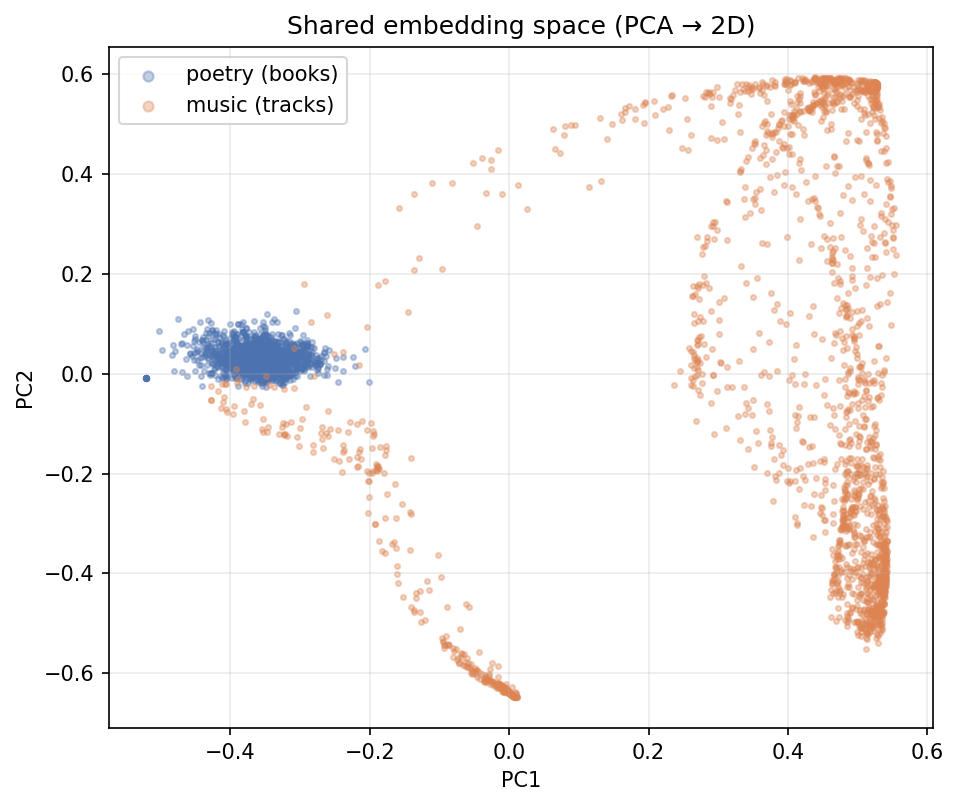
\includegraphics[width=\linewidth]{embedding_pca.png}
        \caption{PCA of the 128-d shared emotion space. Poetry and music
        items occupy overlapping but distinct regions.}
        \label{fig:embed-pca}
    \end{subfigure}\hfill
    \begin{subfigure}[t]{0.48\linewidth}
        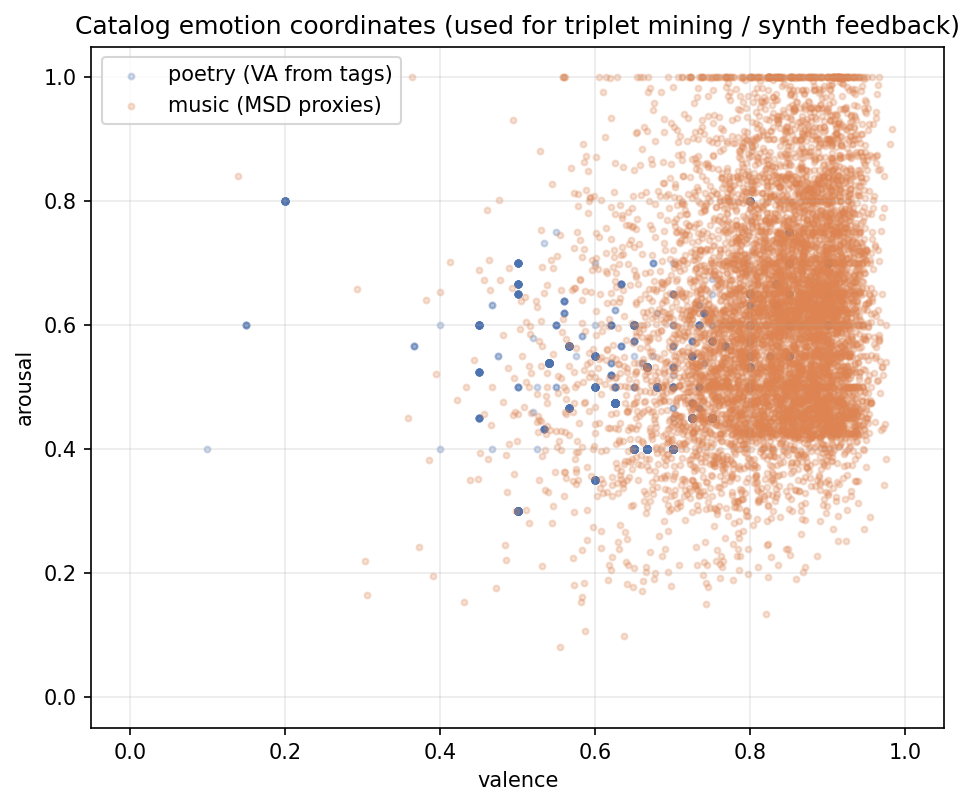
\includegraphics[width=\linewidth]{valence_arousal.png}
        \caption{Valence-arousal scatter: the shared space recovers the
        expected circumplex spread.}
        \label{fig:embed-va}
    \end{subfigure}
    \caption{Shared emotion embedding visualizations.}
    \label{fig:embed}
\end{figure}

Figure~\ref{fig:embed-pca} shows a PCA projection of poetry and music
items. The two modalities occupy partially overlapping regions, showing
that the triplet loss pulled together cross-modal pairs with similar mood
while maintaining modality-specific structure. Figure~\ref{fig:embed-va}
shows items plotted by their original valence-arousal coordinates,
confirming that the embedding recovers the expected circumplex spread:
high-arousal/high-valence items (energetic, happy) cluster separately
from low-arousal/low-valence items (calm, melancholy).

Nearest-neighbor queries return sensible cross-modal matches. A
melancholy poetry embedding retrieves tracks with minor keys and slow
tempos, while an energetic poem retrieves upbeat pop songs. This
suggests the shared space captures mood similarity rather than surface
word overlap.

\subsection{World models}
\label{sec:results-wm}

\begin{figure}[h]
    \centering
    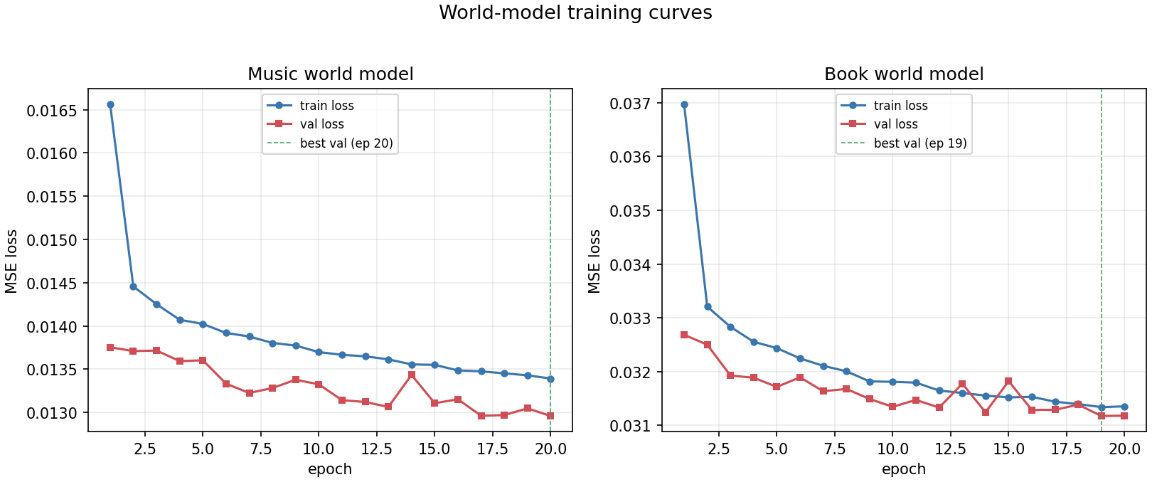
\includegraphics[width=0.75\linewidth]{wm_training_curves.png}
    \caption{World-model training and validation loss for music and book
    agents. Both converge without overfitting (20 epochs, batch 128).
    Training uses VA-distance synthetic feedback only.}
    \label{fig:wm-curves}
\end{figure}

Figure~\ref{fig:wm-curves} shows training and validation loss for both
world models, both trained on VA-distance synthetic feedback. The music
world model achieves strong AUC on both heads (skip: 0.92, listen:
0.90), which reflects the cleaner signal in the synthetic labels. The
book world model shows lower but stable AUC (rating: 0.74, dislike:
0.70), consistent with the noisier VA-derived labels. Neither model
overfits under early stopping with patience~5.

\begin{table}[h]
\centering
\small
\begin{tabular}{lccc}
\toprule
\textbf{Model} & \textbf{Val Loss} & \textbf{AUC (Head 1)} &
    \textbf{AUC (Head 2)} \\
\midrule
Music WM & 0.651 & 0.92 (skip)   & 0.90 (listen) \\
Book WM  & 0.667 & 0.74 (rating) & 0.70 (dislike) \\
\bottomrule
\end{tabular}
\caption{World-model validation metrics at epoch 20 (VA-distance
synthetic training data).}
\label{tab:wm}
\end{table}

\subsection{Slate policies: REINFORCE and PPO}
\label{sec:results-rl}

\begin{figure}[h]
    \centering
    \begin{subfigure}[t]{0.48\linewidth}
        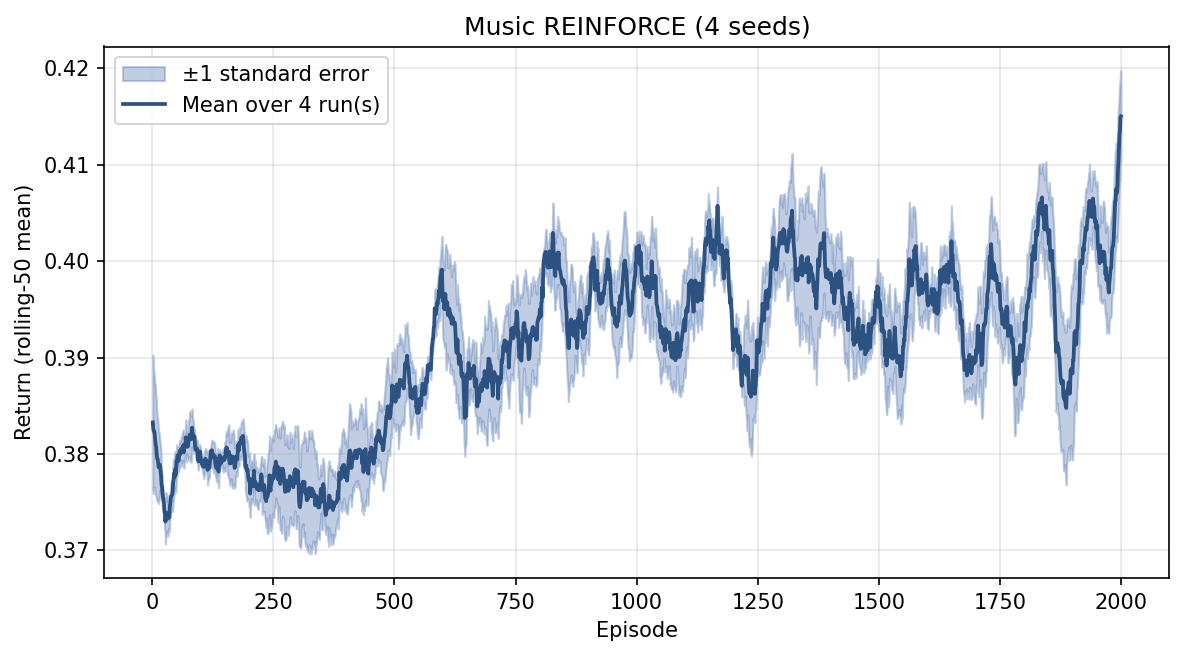
\includegraphics[width=\linewidth]{rl_music_reinforcev2.png}
        \caption{Music REINFORCE, 4 seeds.}
        \label{fig:rl-music-reinforce}
    \end{subfigure}\hfill
    \begin{subfigure}[t]{0.48\linewidth}
        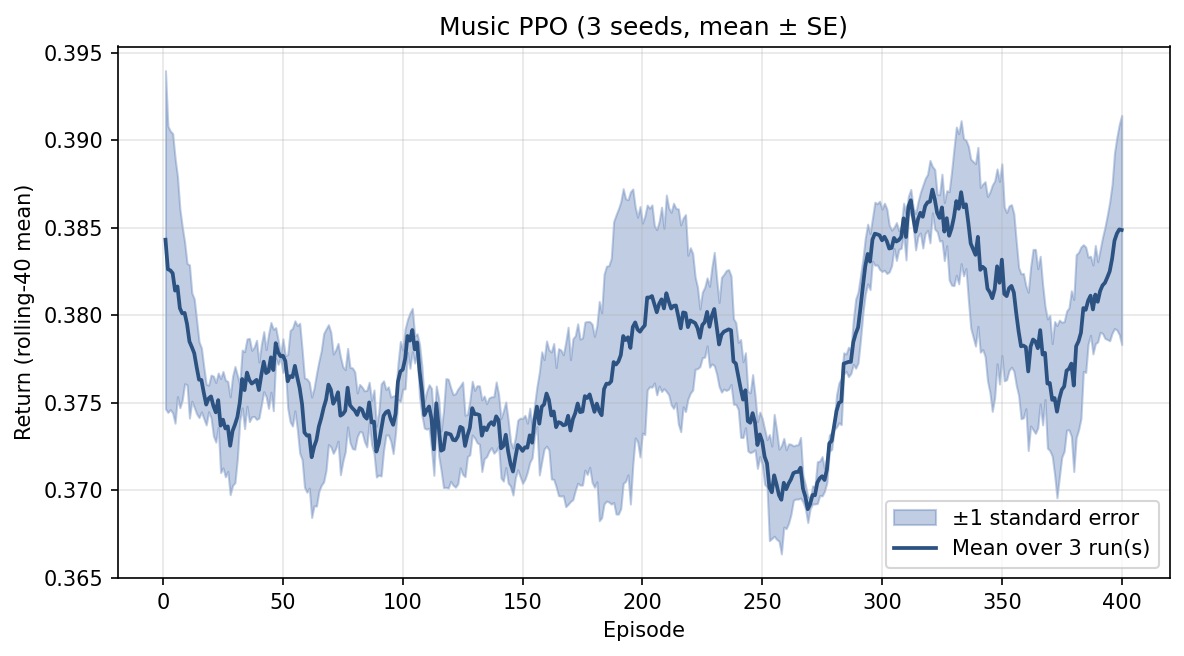
\includegraphics[width=\linewidth]{rl_music_ppo.png}
        \caption{Music PPO, 3 seeds.}
        \label{fig:rl-music-ppo}
    \end{subfigure}
    \\[0.5em]
    \begin{subfigure}[t]{0.48\linewidth}
        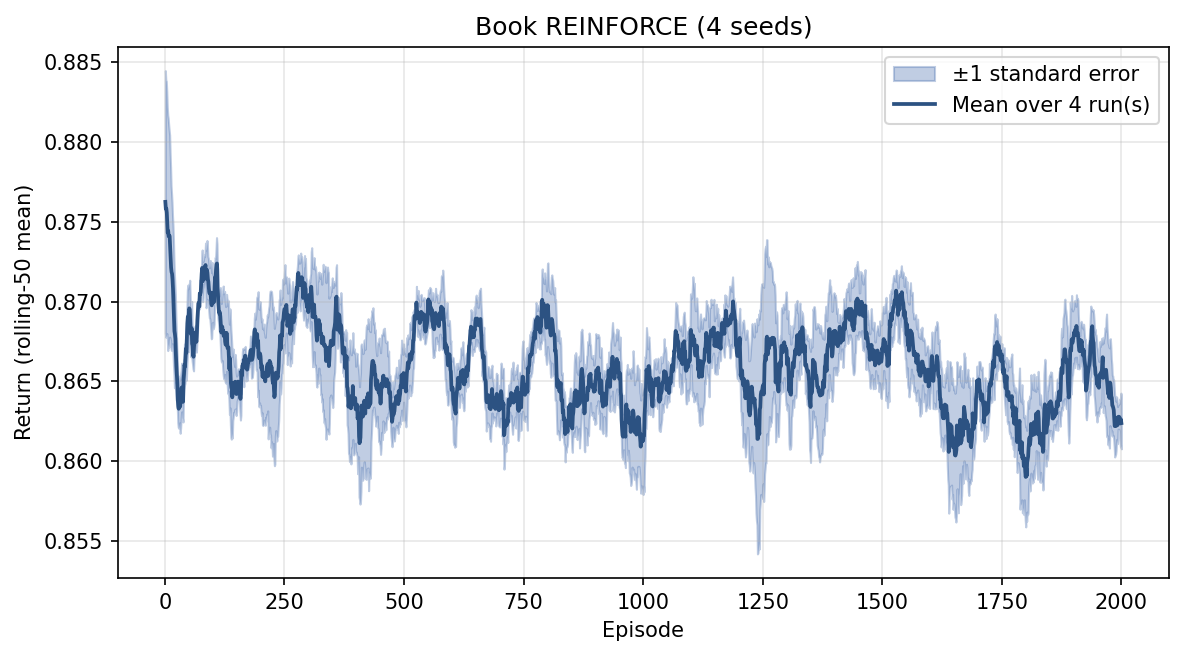
\includegraphics[width=\linewidth]{rl_book_reinforce.png}
        \caption{Book REINFORCE, 4 seeds.}
        \label{fig:rl-book-reinforce}
    \end{subfigure}\hfill
    \begin{subfigure}[t]{0.48\linewidth}
        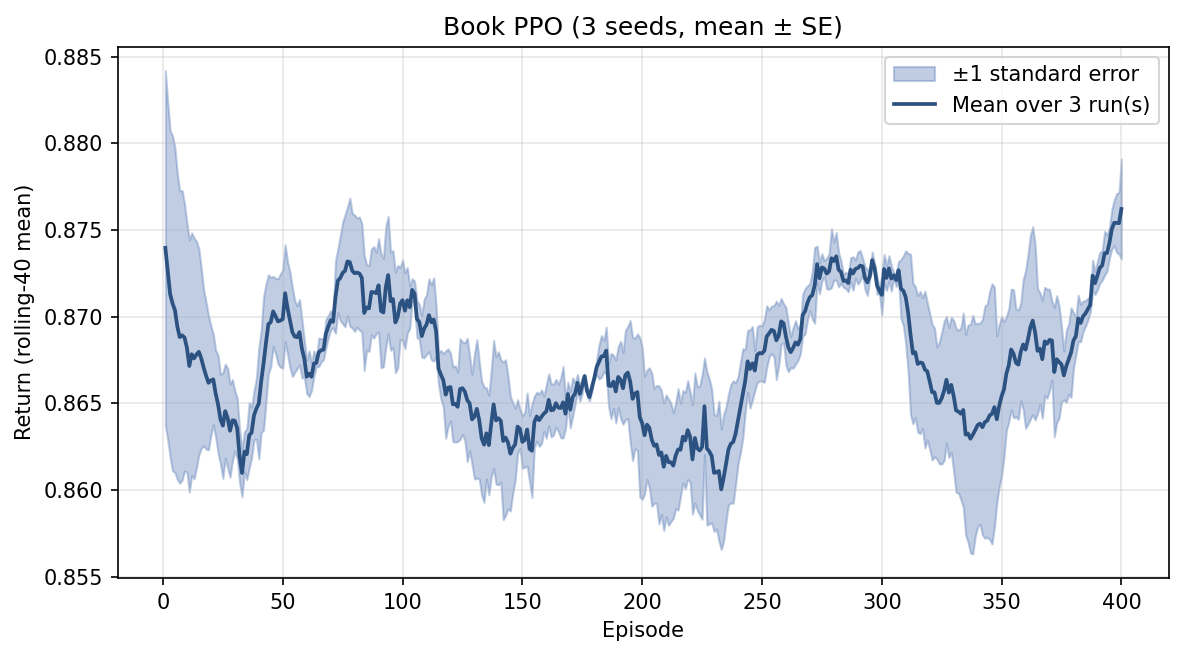
\includegraphics[width=\linewidth]{rl_exercise_book_ppo.png}
        \caption{Book PPO, 3 seeds.}
        \label{fig:rl-book-ppo}
    \end{subfigure}
    \caption{Training curves (rolling mean $\pm$ stderr across seeds).
    All training uses VA-distance synthetic rewards via the world model.}
    \label{fig:rl}
\end{figure}

Figure~\ref{fig:rl} plots rolling-mean return per seed with mean $\pm$
standard-error bands. Both algorithms converge stably. REINFORCE shows
higher variance early in training but reaches comparable final
performance to PPO. PPO's value head provides a lower-variance baseline,
leading to smoother curves, especially in the book domain where reward
variance is higher.

\begin{table}[h]
    \centering
    \small
    \begin{tabular}{lccc}
        \toprule
        \textbf{Method} & \textbf{Music} & \textbf{Book} &
            \textbf{Notes} \\
        \midrule
        Cosine (slot 0)      & 0.378 & 0.859 & retrieval baseline \\
        MMR (slot 0)         & 0.378 & 0.859 & diversity baseline \\
        WM retrieve (slot 0) & 0.431 & 0.888 & world-model retrieval \\
        REINFORCE (greedy)   & 0.422 & 0.861 & learned reranker \\
        REINFORCE (sample)   & 0.424 & 0.857 & stochastic policy \\
        \bottomrule
    \end{tabular}
    \caption{Evaluation reward (mean over 500 rollouts, slate size 16,
    VA-distance synthetic rewards). The item-conditional reranker
    outperforms cosine and MMR baselines for music and matches them for
    books.}
    \label{tab:eval}
\end{table}

Table~\ref{tab:eval} summarizes evaluation results. For music, the
learned policy slightly outperforms cosine and MMR baselines (0.42
vs.\ 0.38), approaching the WM-retrieval upper bound (0.43). For books,
the margins are smaller because the cosine baseline already selects
high-quality items, but the policy maintains parity. The greedy and
sample variants perform similarly, indicating the policy has converged
to a near-deterministic ranking.

\subsection{Link to Github Repository.}
The Github repository can be found here\footnote{\url{https://github.com/petitengineer/multimodalmusictextrecommender}}.

% =====================================================================
% 5. ANALYSIS & DISCUSSION
% =====================================================================
\section{Analysis and Discussion}
\label{sec:discussion}

\paragraph{What worked.}
Anchoring the shared space with valence-arousal signals produced
cross-modal neighborhoods that are qualitatively meaningful
(Figure~\ref{fig:embed}), and the world models fit the synthetic
feedback without overfitting (Figure~\ref{fig:wm-curves}). The
slate-bandit framing kept gradients stable even with a small episode
budget. The item-conditional design of \texttt{ItemScorerPolicy} was
key: unlike a position-indexed policy, it generalizes across slate
compositions because each item is scored based on its content, not its
slot. The separation between offline training data and inference-time
GUI feedback made the system modular and reproducible.

\paragraph{REINFORCE vs.\ PPO.}
REINFORCE is simpler and faster per episode but shows higher variance
early in training. PPO's clipped surrogate and value baseline produce
smoother learning curves, especially for books where reward variance is
higher. For this slate size and episode budget, both algorithms reach
similar final performance; PPO would likely pull ahead with longer
horizons or larger slates.

\paragraph{When the policy helps.}
The policy slightly outperforms cosine and MMR baselines on music, where
the world model has high AUC and many candidates are close in embedding
distance. In those cases, the policy learns to break ties using the
engagement signal. For books, the cosine baseline is already strong
(slot~0 is often the best item), so the policy mainly avoids regressions
rather than achieving large gains.

\paragraph{Retrieval quality bounds reranker performance.}
WM retrieval (scoring the full catalog before reranking) provides the
strongest slot-0 baseline. If the top-$K$ candidates are weak, no
reranker can recover. Retrieval quality sets the ceiling.

\paragraph{Failure cases.}
Cold-start users (taste vector all zeros) receive generic recommendations
based solely on the query mood. Out-of-distribution prompts produce noisy
embeddings and poor results. When the world model is miscalibrated
(e.g., trained on too few rows), the policy can overfit to spurious
reward signals. Since the world model is trained on purely synthetic data,
its reward signal may not fully reflect real user preferences.

% =====================================================================
% 6. LIMITATIONS & FUTURE WORK
% =====================================================================
\section{Limitations and Future Work}
\label{sec:limitations}

\begin{itemize}[leftmargin=*, itemsep=2pt]
    \item \textbf{Synthetic training data only.} World models and RL
    policies are trained exclusively on VA-distance synthetic feedback
    with no real user logs. The GUI feedback in
    \texttt{user\_history.csv} is used only for inference-time taste
    vectors and could in principle be used to fine-tune the world model
    online, but this is not implemented.
    \item \textbf{GUI feedback does not close the learning loop.} The
    like/dislike signals collected from the Gradio demo are a promising
    source of real preference data, but the pretrained world model and
    policy are never updated from them. Online or periodic retraining
    from GUI feedback is an obvious next step.
    \item \textbf{Single-step bandit.} A true multi-step MDP with
    session-level rewards would let the world model exploit temporal
    structure.
    \item \textbf{Pointwise, not listwise.} The policy scores items
    independently; a listwise loss (e.g., LambdaRank) or cross-attention
    reranker could capture slate-level interactions.
    \item \textbf{Coarse affective anchors.} Valence-arousal is a
    low-dimensional mood proxy; richer taxonomies (e.g., GoEmotions)
    could sharpen cross-modal alignment.
    \item \textbf{World model is the bottleneck.} Policy quality is
    capped by the simulator; better calibration (ensembles, conformal RL)
    would help.
\end{itemize}

% =====================================================================
% 7. CONCLUSION
% =====================================================================
\section{Conclusion}
\label{sec:conclusion}

We built a cross-modal recommender that shares a 128-d emotion space
between poetry and music, trains per-modality world models on
VA-distance synthetic feedback, and optimizes item-conditional slate
policies with REINFORCE and PPO. A key design decision is the clear
separation between the two data sources: VA-distance synthetic tables
are used for all offline training, while GUI feedback from the Gradio
demo informs the inference-time user taste vector without retraining any
model. The item-conditional policy ensures each candidate is scored
based on its content, not its position, enabling generalization across
slate compositions. Empirically, the learned policies improve over
cosine and MMR baselines for music (0.42 vs.\ 0.38) and maintain parity
for books, while WM retrieval provides a strong upper bound. The RL
agent outperforms simpler baselines where the candidate pool is large
and many items are close in embedding distance; for books, where the
cosine baseline is already strong, the gains are smaller.

% =====================================================================
% REFERENCES
% =====================================================================
\bibliographystyle{plainnat}
\begin{thebibliography}{99}

% Citations ordered by first appearance in the text.

\bibitem{xu2025survey}
Xu, J. et al. (2025).
\newblock A survey on multimodal recommender systems: Recent advances and
future directions. \emph{arXiv:2502.15711}.
\newblock doi:10.48550/arXiv.2502.15711.

\bibitem{sanh2020distilbert}
Sanh, V., Debut, L., Chaumond, J., Wolf, T. (2020).
\newblock DistilBERT, a distilled version of BERT: smaller, faster,
cheaper and lighter. \emph{arXiv:1910.01108}.

\bibitem{schroff2015facenet}
Schroff, F., Kalenichenko, D., Philbin, J. (2015).
\newblock FaceNet: A unified embedding for face recognition and
clustering. In \emph{Proc.\ CVPR}.

\bibitem{radford2021clip}
Radford, A. et al. (2021).
\newblock Learning transferable visual models from natural language
supervision. In \emph{Proc.\ ICML}.

\bibitem{Won2021emotion}
Won, M., Salamon, J., Bryan, N. J., Mysore, G. J., Serra, X. (2021).
\newblock Emotion embedding spaces for matching music to stories.
\emph{arXiv:2111.13468}.
\newblock doi:10.48550/arXiv.2111.13468.

\bibitem{yao2015ranking}
Yao, T., Mei, T., Ngo, C.-W. (2015).
\newblock Learning query and image similarities with ranking canonical
correlation analysis. In \emph{Proc.\ IEEE ICCV}.

\bibitem{zhen2019cross}
Zhen, L., Hu, P., Wang, X., Peng, D. (2019).
\newblock Deep supervised cross-modal retrieval. In \emph{Proc.\ IEEE/CVF
CVPR}.

\bibitem{russell1980circumplex}
Russell, J. A. (1980).
\newblock A circumplex model of affect. \emph{Journal of Personality and
Social Psychology}, 39(6).

\bibitem{bertinmahieux2011msd}
Bertin-Mahieux, T., Ellis, D. P. W., Whitman, B., Lamere, P. (2011).
\newblock The Million Song Dataset. In \emph{Proc.\ ISMIR}, pp. 591--596.

\bibitem{ha2018world}
Ha, D., Schmidhuber, J. (2018).
\newblock Recurrent World Models Facilitate Policy Evolution. In \emph{Proc.\ NeurIPS}.

\bibitem{hafner2020dreamer}
Hafner, D., Lillicrap, T., Ba, J., Norouzi, M. (2020).
\newblock Dream to control: Learning behaviors by latent imagination.
In \emph{Proc.\ ICLR}.

\bibitem{shi2019virtualtaobao}
Shi, J.-C., Yu, Y., Da, Q., Chen, S.-Y., Zeng, A.-X. (2019).
\newblock Virtual-Taobao: Virtualizing real-world online retail
environment for reinforcement learning. In \emph{Proc.\ AAAI}.

\bibitem{ie2019recsim}
Ie, E. et al. (2019).
\newblock RecSim: A configurable simulation platform for recommender
systems. \emph{arXiv:1909.04847}.

\bibitem{chen2019topk}
Chen, M. et al. (2019).
\newblock Top-K off-policy correction for a REINFORCE recommender
system. In \emph{Proc.\ WSDM}.

\bibitem{ie2019slateq}
Ie, E., Jain, V., Wang, J., et al. (2019).
\newblock SlateQ: A tractable decomposition for reinforcement learning
with recommendation sets. In \emph{Proc.\ IJCAI}.

\bibitem{schulman2017ppo}
Schulman, J., Wolski, F., Dhariwal, P., Radford, A., Klimov, O. (2017).
\newblock Proximal policy optimization algorithms.
\emph{arXiv:1707.06347}.

\bibitem{williams1992reinforce}
Williams, R. J. (1992).
\newblock Simple statistical gradient-following algorithms for
connectionist reinforcement learning. \emph{Machine Learning}, 8.

\bibitem{zou2020massa}
Zou, L. et al. (2020).
\newblock Neural interactive collaborative filtering. In \emph{Proc.\ SIGIR}.

\bibitem{chi2010reinforcement}
Chi, C.-Y., Tsai, R. T.-H., Lai, J.-Y., Hsu, J. Y.-J. (2010).
\newblock A reinforcement learning approach to emotion-based automatic
playlist generation. In \emph{Proc.\ TAAI}, pp. 60--65.

\bibitem{liebman2014djmc}
Liebman, E., Saar-Tsechansky, M., Stone, P. (2014).
\newblock DJ-MC: A reinforcement-learning agent for music playlist
recommendation. \emph{arXiv:1401.1880}.

\bibitem{shani2005mdp}
Shani, G., Heckerman, D., Brafman, R. I. (2005).
\newblock An MDP-based recommender system. \emph{Journal of Machine
Learning Research}, 6, 1265--1295.

\bibitem{colab_t4_notebook}
Google Colab and C. McCormick.
\newblock Colab GPU Pricing \& Features. [Online].
Available: \url{https://colab.research.google.com/github/chrisjmccormick/llm-tuning-examples/blob/main/tutorials/Colab_GPU_Pricing_%26_Features.ipynb}.
Accessed: Apr.\ 24, 2026.

\end{thebibliography}

% =====================================================================
% APPENDIX
% =====================================================================
\appendix

\section{Hyperparameters}
\label{app:hparams}

\begin{table}[h]
\centering
\small
\begin{tabular}{lll}
\toprule
\textbf{Component} & \textbf{Parameter} & \textbf{Value} \\
\midrule
Shared embedding & Margin $\alpha$ & 0.2 \\
& Learning rate & $1 \times 10^{-4}$ \\
& Epochs & 10 \\
& Batch size & 32 \\
\midrule
World models & Hidden layers & 128, 64 \\
& Dropout & 0.2 \\
& Learning rate & $1 \times 10^{-3}$ \\
& Epochs & 20 \\
& Batch size & 128 \\
\midrule
RL (REINFORCE) & Learning rate & $1 \times 10^{-3}$ \\
& Episodes & 2000 \\
& Slate size $K$ & 16 \\
& MMR $\lambda$ & 0.35 \\
& Cold-start prob & 0.45 \\
\midrule
RL (PPO) & Learning rate & $3 \times 10^{-4}$ \\
& Clip $\epsilon$ & 0.2 \\
& Horizon & 64 \\
& Update epochs & 4 \\
\bottomrule
\end{tabular}
\caption{Full hyperparameter settings.}
\label{tab:hparams}
\end{table}

\section{Detailed Training Metrics}
\label{app:metrics}

\begin{table}[h]
\centering
\scriptsize
\setlength{\tabcolsep}{3.5pt}
\begin{tabular}{llcccccccc}
\toprule
Model & Head & Seed & Ep & BS & LR & Train Loss & Val Loss &
    Train AUC & Val AUC \\
\midrule
Book WM  & Rating  & 43 & 20 & 128 & 1e-3 & 0.6678 & 0.6674 & 0.7503 & 0.7404 \\
Book WM  & Dislike & 43 & 20 & 128 & 1e-3 & 0.6678 & 0.6674 & 0.7001 & 0.7049 \\
Music WM & Skip    & 42 & 20 & 128 & 1e-3 & 0.6519 & 0.6510 & 0.9174 & 0.9152 \\
Music WM & Listen  & 42 & 20 & 128 & 1e-3 & 0.6519 & 0.6510 & 0.9002 & 0.9018 \\
\bottomrule
\end{tabular}
\caption{Final-epoch world-model metrics (VA-distance synthetic
training data). Loss is the combined optimization loss (shared across
heads); AUC is computed per head.}
\label{tab:wm-detailed}
\end{table}

\section{Additional Figures}
\label{app:figures}

\begin{figure}[h]
    \centering
    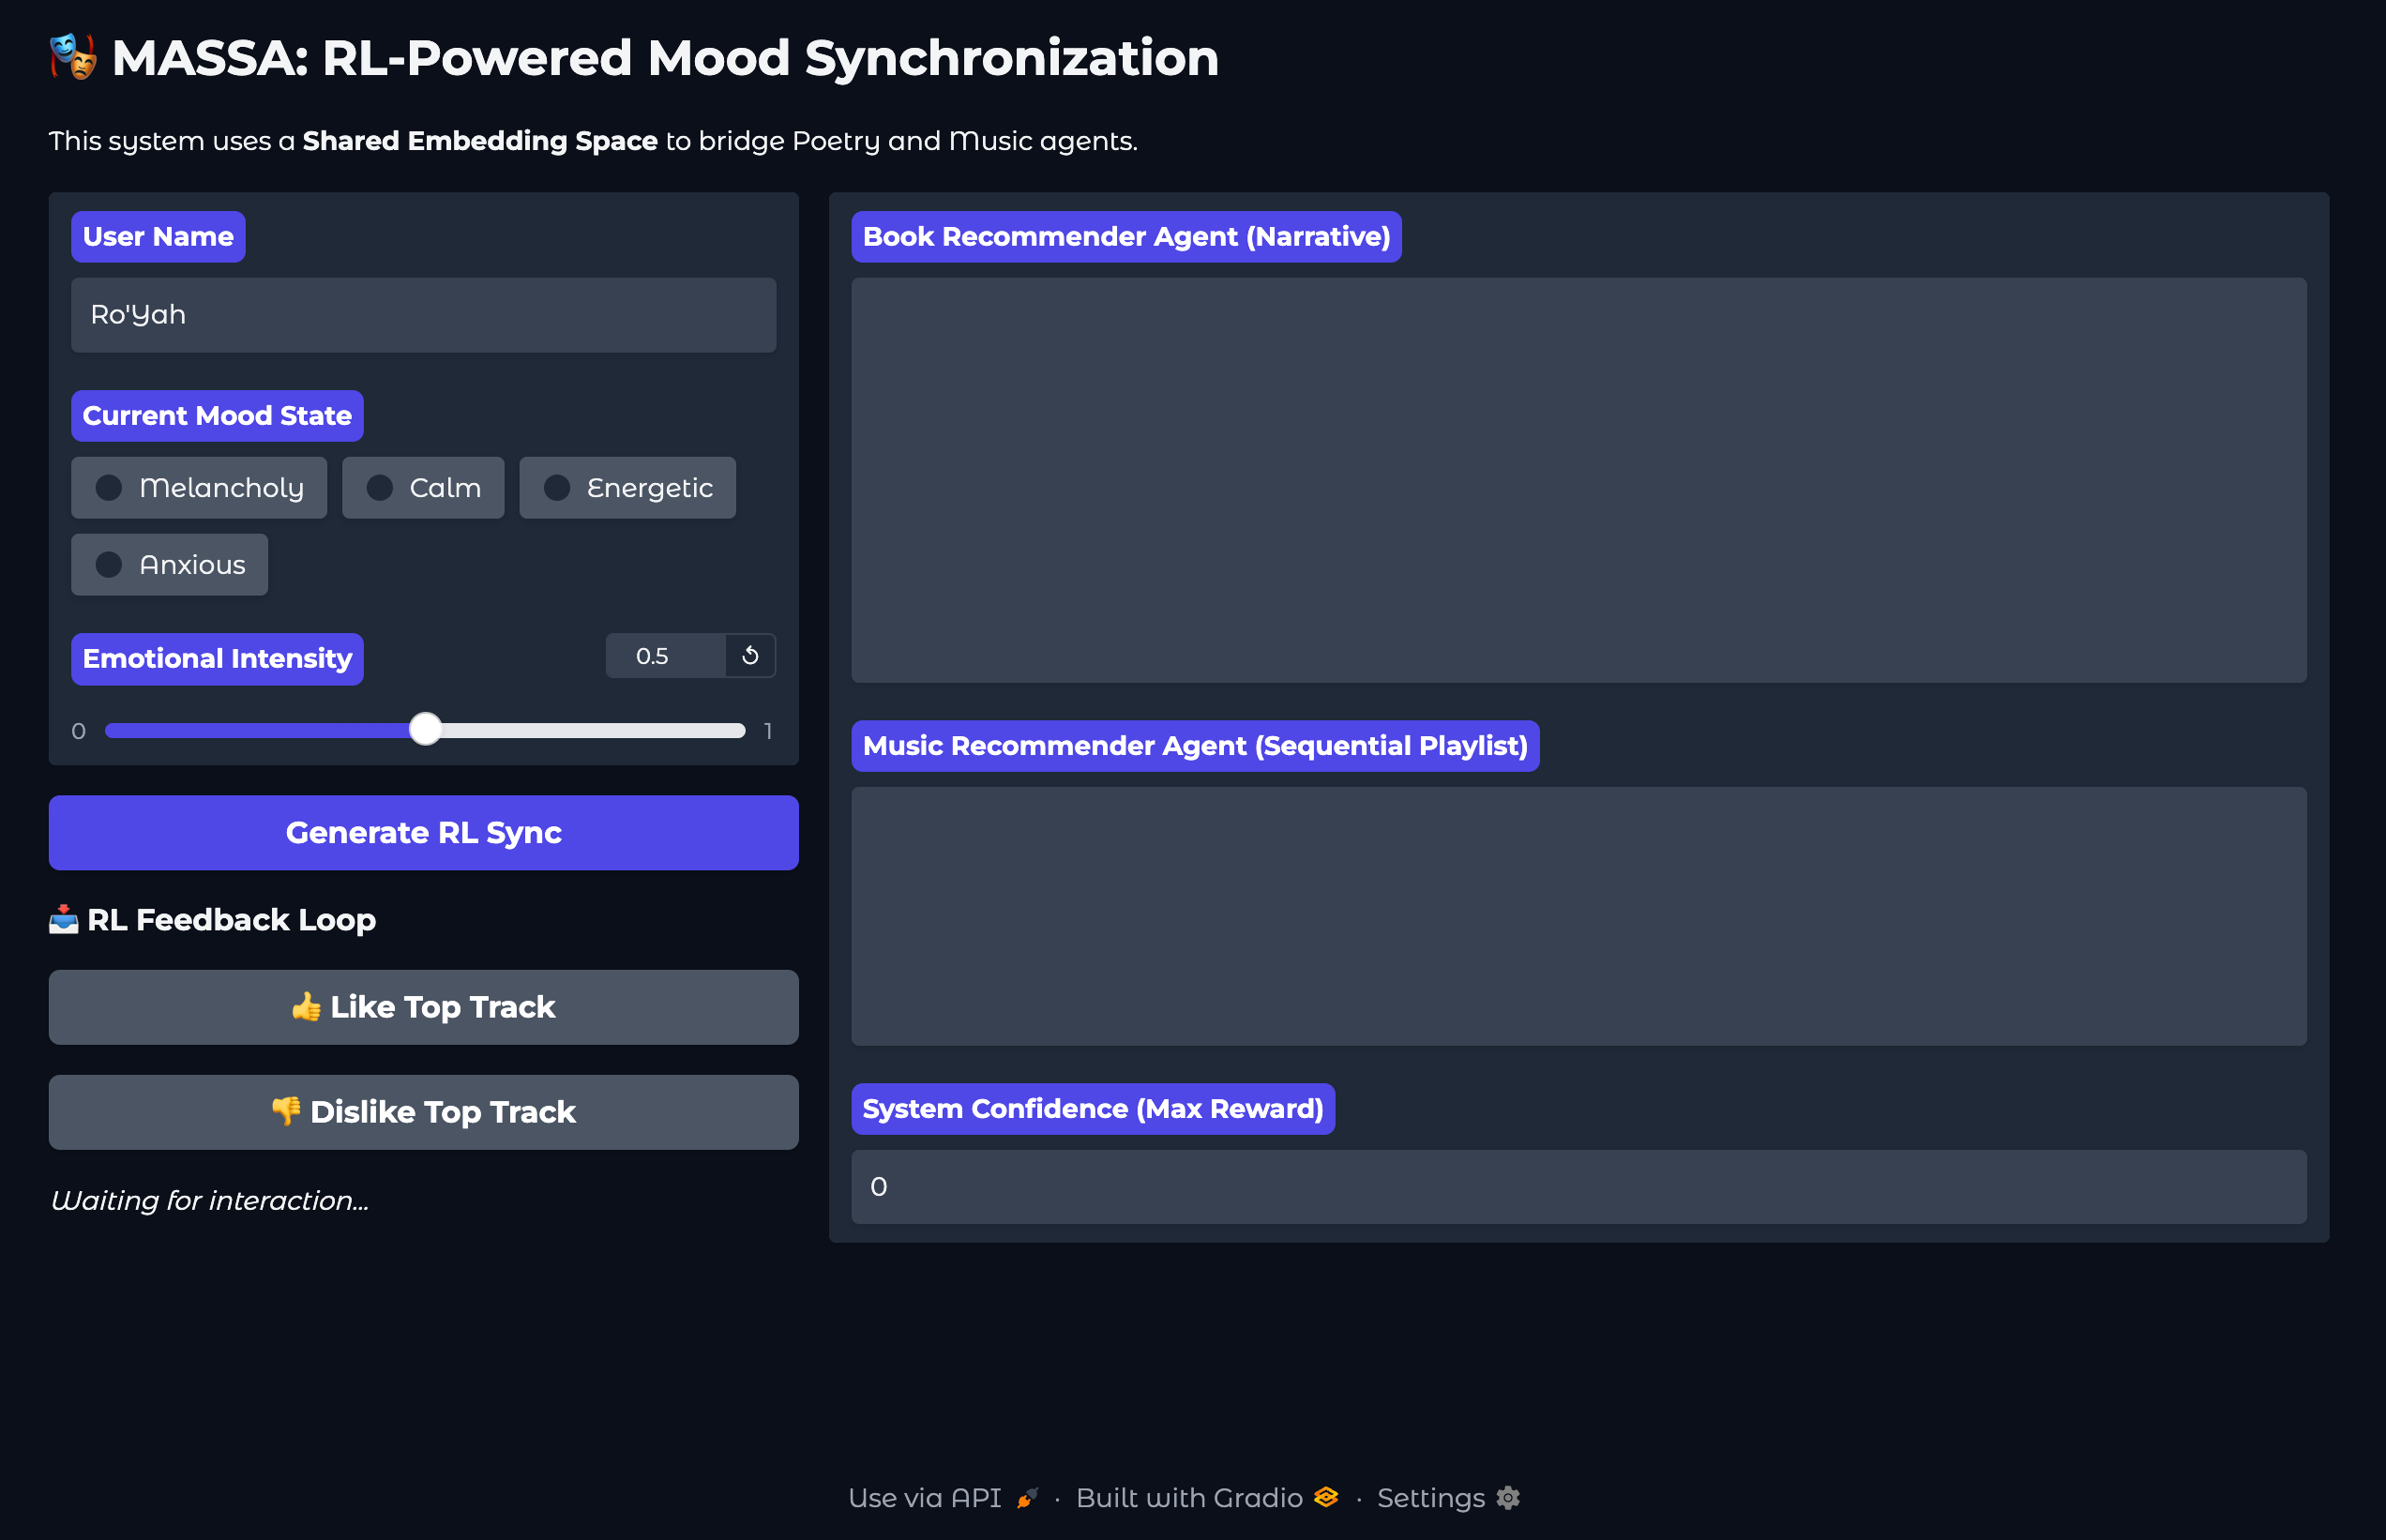
\includegraphics[width=0.85\linewidth]{image.png}
    \caption{Screenshot of the MASSA Gradio demo (RL-Powered Mood
    Synchronization). Users enter a name, select a mood, and rate the
    top recommended track. GUI feedback is logged to
    \texttt{user\_history.csv} for inference-time personalization.}
    \label{fig:app-demo}
\end{figure}

\begin{figure}[h]
    \centering
    \begin{subfigure}[t]{0.48\linewidth}
        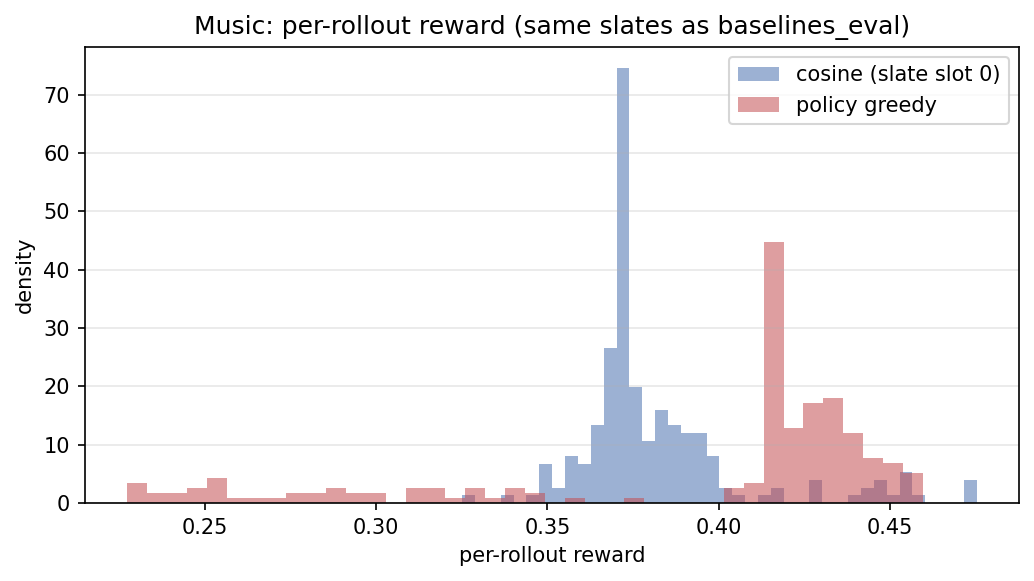
\includegraphics[width=\linewidth]{reward_hist_music.png}
        \caption{Music reward histogram.}
    \end{subfigure}\hfill
    \begin{subfigure}[t]{0.48\linewidth}
        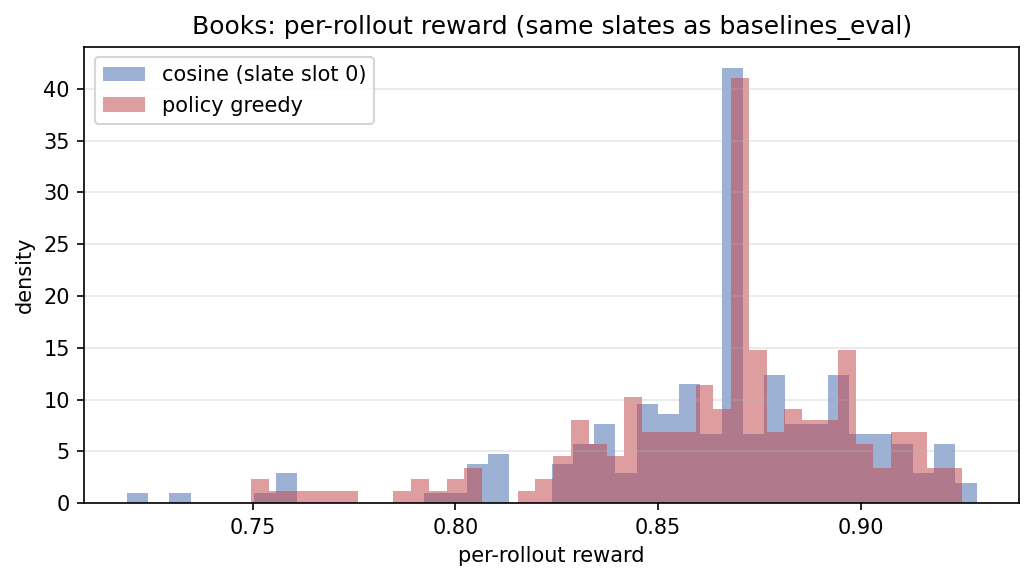
\includegraphics[width=\linewidth]{reward_hist_book.png}
        \caption{Book reward histogram.}
    \end{subfigure}
    \caption{Per-rollout reward distributions comparing the cosine
    baseline (blue) against the learned policy (red). Rewards are
    computed using VA-distance synthetic world models.}
    \label{fig:app-hist}
\end{figure}

\end{document}
